\documentclass[twoside]{book}

% Packages required by doxygen
\usepackage{fixltx2e}
\usepackage{calc}
\usepackage{doxygen}
\usepackage[export]{adjustbox} % also loads graphicx
\usepackage{graphicx}
\usepackage[utf8]{inputenc}
\usepackage{makeidx}
\usepackage{multicol}
\usepackage{multirow}
\PassOptionsToPackage{warn}{textcomp}
\usepackage{textcomp}
\usepackage[nointegrals]{wasysym}
\usepackage[table]{xcolor}

% Font selection
\usepackage[T1]{fontenc}
\usepackage[scaled=.90]{helvet}
\usepackage{courier}
\usepackage{amssymb}
\usepackage{sectsty}
\renewcommand{\familydefault}{\sfdefault}
\allsectionsfont{%
  \fontseries{bc}\selectfont%
  \color{darkgray}%
}
\renewcommand{\DoxyLabelFont}{%
  \fontseries{bc}\selectfont%
  \color{darkgray}%
}
\newcommand{\+}{\discretionary{\mbox{\scriptsize$\hookleftarrow$}}{}{}}

% Page & text layout
\usepackage{geometry}
\geometry{%
  a4paper,%
  top=2.5cm,%
  bottom=2.5cm,%
  left=2.5cm,%
  right=2.5cm%
}
\tolerance=750
\hfuzz=15pt
\hbadness=750
\setlength{\emergencystretch}{15pt}
\setlength{\parindent}{0cm}
\setlength{\parskip}{3ex plus 2ex minus 2ex}
\makeatletter
\renewcommand{\paragraph}{%
  \@startsection{paragraph}{4}{0ex}{-1.0ex}{1.0ex}{%
    \normalfont\normalsize\bfseries\SS@parafont%
  }%
}
\renewcommand{\subparagraph}{%
  \@startsection{subparagraph}{5}{0ex}{-1.0ex}{1.0ex}{%
    \normalfont\normalsize\bfseries\SS@subparafont%
  }%
}
\makeatother

% Headers & footers
\usepackage{fancyhdr}
\pagestyle{fancyplain}
\fancyhead[LE]{\fancyplain{}{\bfseries\thepage}}
\fancyhead[CE]{\fancyplain{}{}}
\fancyhead[RE]{\fancyplain{}{\bfseries\leftmark}}
\fancyhead[LO]{\fancyplain{}{\bfseries\rightmark}}
\fancyhead[CO]{\fancyplain{}{}}
\fancyhead[RO]{\fancyplain{}{\bfseries\thepage}}
\fancyfoot[LE]{\fancyplain{}{}}
\fancyfoot[CE]{\fancyplain{}{}}
\fancyfoot[RE]{\fancyplain{}{\bfseries\scriptsize Generated by Doxygen }}
\fancyfoot[LO]{\fancyplain{}{\bfseries\scriptsize Generated by Doxygen }}
\fancyfoot[CO]{\fancyplain{}{}}
\fancyfoot[RO]{\fancyplain{}{}}
\renewcommand{\footrulewidth}{0.4pt}
\renewcommand{\chaptermark}[1]{%
  \markboth{#1}{}%
}
\renewcommand{\sectionmark}[1]{%
  \markright{\thesection\ #1}%
}

% Indices & bibliography
\usepackage{natbib}
\usepackage[titles]{tocloft}
\setcounter{tocdepth}{3}
\setcounter{secnumdepth}{5}
\makeindex

% Hyperlinks (required, but should be loaded last)
\usepackage{ifpdf}
\ifpdf
  \usepackage[pdftex,pagebackref=true]{hyperref}
\else
  \usepackage[ps2pdf,pagebackref=true]{hyperref}
\fi
\hypersetup{%
  colorlinks=true,%
  linkcolor=blue,%
  citecolor=blue,%
  unicode%
}

% Custom commands
\newcommand{\clearemptydoublepage}{%
  \newpage{\pagestyle{empty}\cleardoublepage}%
}

\usepackage{caption}
\captionsetup{labelsep=space,justification=centering,font={bf},singlelinecheck=off,skip=4pt,position=top}

%===== C O N T E N T S =====

\begin{document}

% Titlepage & ToC
\hypersetup{pageanchor=false,
             bookmarksnumbered=true,
             pdfencoding=unicode
            }
\pagenumbering{roman}
\begin{titlepage}
\vspace*{7cm}
\begin{center}%
{\Large My Project }\\
\vspace*{1cm}
{\large Generated by Doxygen 1.8.11}\\
\end{center}
\end{titlepage}
\clearemptydoublepage
\tableofcontents
\clearemptydoublepage
\pagenumbering{arabic}
\hypersetup{pageanchor=true}

%--- Begin generated contents ---
\chapter{File Index}
\section{File List}
Here is a list of all files with brief descriptions\+:\begin{DoxyCompactList}
\item\contentsline{section}{\hyperlink{Lab1_8c}{Lab1.\+c} }{\pageref{Lab1_8c}}{}
\end{DoxyCompactList}

\chapter{File Documentation}
\hypertarget{PizzaOrder_8cpp}{}\section{Pizza\+Order.\+cpp File Reference}
\label{PizzaOrder_8cpp}\index{Pizza\+Order.\+cpp@{Pizza\+Order.\+cpp}}
{\ttfamily \#include $<$iostream$>$}\\*
{\ttfamily \#include $<$string$>$}\\*
Include dependency graph for Pizza\+Order.\+cpp\+:
\nopagebreak
\begin{figure}[H]
\begin{center}
\leavevmode
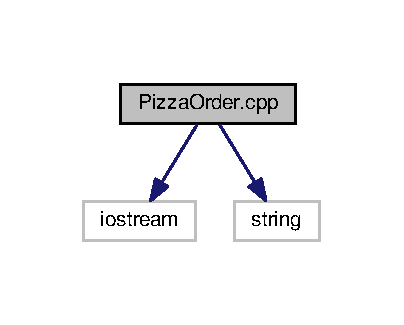
\includegraphics[width=194pt]{PizzaOrder_8cpp__incl}
\end{center}
\end{figure}
\subsection*{Functions}
\begin{DoxyCompactItemize}
\item 
int \hyperlink{PizzaOrder_8cpp_ae66f6b31b5ad750f1fe042a706a4e3d4}{main} ()
\end{DoxyCompactItemize}


\subsection{Function Documentation}
\index{Pizza\+Order.\+cpp@{Pizza\+Order.\+cpp}!main@{main}}
\index{main@{main}!Pizza\+Order.\+cpp@{Pizza\+Order.\+cpp}}
\subsubsection[{\texorpdfstring{main()}{main()}}]{\setlength{\rightskip}{0pt plus 5cm}int main (
\begin{DoxyParamCaption}
{}
\end{DoxyParamCaption}
)}\hypertarget{PizzaOrder_8cpp_ae66f6b31b5ad750f1fe042a706a4e3d4}{}\label{PizzaOrder_8cpp_ae66f6b31b5ad750f1fe042a706a4e3d4}

\begin{DoxyCode}
6 \{
7    cout.setf(ios::fixed); \textcolor{comment}{// These three sets of lines tell the computer to                                
                                                                                                       }
8    cout.setf(ios::showpoint); \textcolor{comment}{// output all double numbers so that they                                    
                                                                                                       }
9    cout.precision(2); \textcolor{comment}{// always have 2 decimal points, no more or less                                     
                                                                                                       }
10    \textcolor{keywordtype}{string} name;
11    \textcolor{keywordtype}{int} twelve\_inch, fourteen\_inch;
12    \textcolor{keywordtype}{double} total\_amount, amount\_recieved, change;
13 
14    cout << \textcolor{stringliteral}{"Welcome to Little Italy Pizza\(\backslash\)n"};
15    cout << \textcolor{stringliteral}{"Please enter the customer's FIRST name: "};
16    cin >> name;
17    cout << \textcolor{stringliteral}{"How many 12 inch pizzas are ordered? "};
18    cin >> twelve\_inch;
19    cout << \textcolor{stringliteral}{"How many 14 inch pizzas are ordered? "};
20    cin >> fourteen\_inch;
21 
22    total\_amount = (twelve\_inch * 12.39) + (fourteen\_inch * 15.98);
23    \textcolor{comment}{/* To find the total amount, multiply the amount of 12 inch pizzas and the        amount of 14 inch
       pizzas by how much they cost, and then add the two                                                   }
24 \textcolor{comment}{      numbers together */}
25    cout << \textcolor{stringliteral}{"Total amount due is: $"} << total\_amount << endl;
26    cout << \textcolor{stringliteral}{"The amount recieved from the customer: $"};
27    cin >> amount\_recieved;
28    change = amount\_recieved - total\_amount;
29 
30    cout << endl;
31    cout << \textcolor{stringliteral}{"------------------------------\(\backslash\)n"};
32    cout << \textcolor{stringliteral}{"Receipt by Little Italy Pizza\(\backslash\)n"};
33    cout << \textcolor{stringliteral}{"------------------------------\(\backslash\)n"};
34    cout << \textcolor{stringliteral}{"Customer's First Name: "} << name << endl;
35    cout << \textcolor{stringliteral}{"------------------------------\(\backslash\)n"};
36    cout << \textcolor{stringliteral}{"Pizza    Num    Price\(\backslash\)n"};
37    cout << \textcolor{stringliteral}{"12-in    "} << twelve\_inch << \textcolor{stringliteral}{"      $"} << twelve\_inch*12.39;
38    \textcolor{comment}{// The number of 12 inch pizzas multiplied by the amount one pizza costs                                
                                                                                                       }
39    \textcolor{comment}{// displays the total cost of 12 inch pizzas ordered                                                    
                                                                                                       }
40    cout << endl;
41    cout << \textcolor{stringliteral}{"14-in    "} << fourteen\_inch << \textcolor{stringliteral}{"      $"} << fourteen\_inch*15.98;
42    \textcolor{comment}{// Finding the total cost of 14 inch pizzas is similar to finding the total                             
                                                                                                       }
43    \textcolor{comment}{// cost for 12 inch pizzas                                                                              
                                                                                                       }
44    cout << endl;
45    cout << \textcolor{stringliteral}{"------------------------------\(\backslash\)n"};
46    cout << \textcolor{stringliteral}{"Total:          $"} << total\_amount << endl;
47    cout << \textcolor{stringliteral}{"Recieved:       $"} << amount\_recieved << endl;
48    cout << \textcolor{stringliteral}{"Change:         $"} << change << endl;
49    cout << \textcolor{stringliteral}{"------------------------------\(\backslash\)n"};
50 
51    \textcolor{keywordflow}{return} 0;
52 \}
\end{DoxyCode}

%--- End generated contents ---

% Index
\backmatter
\newpage
\phantomsection
\clearemptydoublepage
\addcontentsline{toc}{chapter}{Index}
\printindex

\end{document}
